\documentclass[uplatex,dvipdfmx]{jsarticle}

\input{"preamble.tex"}

\title{高校数学における「文字」の扱い}

\author{ガオゾウ}



\begin{document}

	\maketitle
	
	\section{はじめに}
	このpdfでは数学における最も基本的な道具である「文字」の扱いに関してまとめていきます。
	
	ここでいう「文字」とは、以下のようなものを指します。
	\begin{itemize}
		\item $ x^2 + 3x + 2 = 0 $における$x$
		\item $ y = x^3 + 3x $における$x,y$
		\item $ a\sin(\theta) + b\cos(\theta) = \sqrt{a^2+b^2}sin(\theta + \alpha) $における$a,b,\theta$
	\end{itemize}
	
	これらは一口に文字といっても、それぞれ異なる扱いをしなくてはなりません。各文字が果たしている役割は(もちろん文脈にもよりますが)異なります。
	
	このpdfでは、これらの文字の意味の違いをある程度整理し、文字の意味がよくわかっていない高校生向けに解説していきたいと思います。
	
	\vspace{1cm}
	
	【お断り】上で挙げた例もそうですが、数式中の文字の役割は、基本的にすべて文脈に依存します。したがって、上のように数式だけ挙げて「これらの文字の意味はすべて異なる」などというのは本当はナンセンスです。また、このpdfでもある程度文字の役割を分類立てて解説しますが、ある一つの文字が様々な役割を担うことは多々あります。例えばある問題に出てきた式中のある文字が、その問題の解答の前半ではAという役割を持っていても、後半ではBという役割を持つ、というようなことは、数式を扱っていれば日常茶飯事です。したがって、すべての文字がこのpdfで紹介した役割にきれいに分類できるわけでもありません。また、ここで紹介する文字の役割はあくまで一つの見方であり、その他の考え方や解釈はいくらでもあります。ここで紹介した文字の扱いのみにとらわれることなく、自由にいろいろと考えていただきたいと思います。
	
	
	\section{文字の役割}
	早速数学における文字の役割をいくつか見ていきましょう。このpdfで紹介するのは以下の3種類です。
	\begin{enumerate}
		\item 具体的な数字の代わりの文字(定数)
		\item 条件を表す文字(未知数)
		\item 関係を表す文字(変数)
	\end{enumerate}
	先の【お断り】のところでも述べた通り、世の中の数式に現れる文字のすべてがこの3つに分類されるわけではないですが、少なくとも高校数学くらいまでなら大体この3つの見方を知っていれば、理解に困ることはないかと思います。

	\subsection{条件を表す文字(未知数)}
	突然ですが、こんな問題を考えてみましょう。
	
	\begin{itembox}[l]{問題1}
		はじめ、たかし君はリンゴをいくつか持っています。たかし君は、友達からリンゴを5個もらった後、リンゴを3個食べました。すると、たかし君が持っているリンゴは4個になりました。
		
		たかし君がはじめに持っていたリンゴはいくつだったでしょうか?
	\end{itembox}

	この問題を解くのは簡単だと思います。たぶんほとんど何も考えなくても、答えは2個だとわかるでしょう。念のため、解答を書いておきます。
	
	\begin{itembox}[l]{解答1-1}
		たかし君の持っているリンゴの変化は、$+5-3 = +2$個である。つまり、リンゴを5個もらって3個食べると、たかし君の持っているリンゴは2個増える。2個増えた結果持っているリンゴが4個になったということは、はじめにたかし君が持っていたリンゴの数は、$4-2 = 2$個である。
	\end{itembox}
	
	問題1はいかにも小学生が解きそうな算数の問題ですが、これをもう少し数学らしく、文字を使って解いてみましょう。
	
	\begin{itembox}[l]{解答1-2}
		たかし君がはじめもっていたリンゴの数を$x$とする。リンゴを5個もらい、3個食べた後のたかし君の持っているリンゴの数は、$x+5-3$である。一方問題文より、たかし君が最後に持っているリンゴの数は4個である。したがってこれらは等しいはずである。
		\begin{equation}
			x+5-3=4 \label{eq:takasi}
		\end{equation}
		この一次方程式を解けば、$x=2$がわかる。すなわち、たかし君がはじめに持っていたリンゴは2個である。
	\end{itembox}
	
	この解答1-2中の文字$x$は、たかし君がはじめにもっていたリンゴの数を表しています。この「たかし君の持っていたリンゴの数」がいくらなのかは、解答1-2のはじめではわかっていません。このような文字を\emp{未知数}と呼びます。\gtb{未知数の値がいくらなのかは私たちにはわかりませんが、それは私たちが知らないだけであって、正しい答えが決まっているのが未知数の最大の特徴です}\footnote{「そのような値が存在しない」という答えになることもあります。しかし、「値があるのかないのか、あるのならその値がいくらなのか」については必ず答えが存在します。ただし、それを私たちが知っているかどうかは全くの別問題です。}。
	
	\begin{tcolorbox}[title=\gtb{未知数}]
		値がいくらなのかはわからないが、正しい答えが決まっているような数の代わりに用いる文字のことを未知数と呼ぶ。
	\end{tcolorbox}
	
	この$x$の値がいくらなのかはわかりませんが、$x$が満たしていなければならない条件が、問題文を読んだ結果わかります。それが式(\ref{eq:takasi})です。この条件を満たすような$x$を見つけられれば、先ほどまで私たちが知らなかった$x$の値の(一つ)を私たちは知ったことになります。
	
	他にもいくつか例を見てみましょう。さすがに先ほどの例では簡単すぎるので、もう少し難しい問題にしてみましょう。
	
	\begin{itembox}[l]{問題2}
		鶴と亀がそれぞれ何匹かいます。すべての鶴と亀の足の合計は20本でした。また、すべての鶴と亀の頭の合計は6つでした。鶴と亀はそれぞれ何匹ずついたでしょうか。
	\end{itembox}
	
	引き続き算数、懐かしのつるかめ算です。これを数学らしく解くと次のようになります。
	
	\begin{itembox}[l]{解答2}
		鶴の数を$x$、亀の数を$y$とする。鶴一匹あたり足の数は2本、亀一匹あたり足の数は4本だから、鶴と亀の足の合計が20本ということは、
		\begin{equation}
			2x+4y = 20
		\end{equation}
		が成り立つということである。一方、鶴と亀の頭の合計が6つということは、
		\begin{equation}
			x+y = 6
		\end{equation}
		が成り立つはずである。
		以上の方程式2つを連立して解けば、$x=2, y=4$がわかる。したがって、鶴の数は2匹、亀の数は4匹である。
	\end{itembox}	
	
	この問題では、鶴の数を$x$、亀の数を$y$とおいています。この$xとy$も、前問と同様に未知数です。この$x$と$y$についても、前問と同様に「その値がいくらなのかはわからないが答えが必ず決まっている」ことに注目してください。
	
	もう一つ未知数の例をあげましょう。
	
	\begin{itembox}[l]{問題3}
		次の$x$に関する方程式を解け。
		\begin{equation}
			x^2+3x+2 = 0 \label{eq:deg2}
		\end{equation}
	\end{itembox}
	
	一気に数学らしくなりました。実はこの式(\ref{eq:deg2})に現れている文字$x$も、未知数です。私たちは、式(\ref{eq:deg2})を満たすような$x$(つまり方程式の解)は(問題を解くまで)知りませんが、その答えは存在します。実際に解いてみましょう。
	
	\begin{itembox}[l]{解答3}
		\begin{align*}
			x^2 + 3x + 2&=0 &因数分解して、\\
			(x+1)(x+2) &= 0 &したがって、\\
			x=-1, -2
		\end{align*}
	\end{itembox}
	
	このように実際に方程式を解くことによって、答えを求めることができました。
	
	最後に、練習問題を出しておきましょう。
	
	\begin{itembox}[l]{練習問題1}
		次の文章と式中に現れる文字x, y, a, bのうち、それぞれの文章について未知数であるものをすべて選びなさい。
		
		\begin{enumerate}
			\item xの方程式 $x^3+4x^2+6x+3 = 0$
			\item 直線$y=3x-1$と曲線$y=\sin(x)$の交点の座標を(a,b)とおくと、
			\begin{equation}
				3a-1 = \sin a = b
			\end{equation}
			が成り立つ。
			\item 直線のグラフを表す式 $y = ax+b$
			\item $x$の二次方程式 $ax^2+bx+c = 0, a\neq 0$
		\end{enumerate}
	\end{itembox}
		
	\subsection{関係を表す文字(変数)}
	前節で扱った未知数は、(私たちが答えを知っているかどうかは別にして)正しい答えが存在するような文字のことをいうのでした。それでは、次の式中に現れる文字$x$を考えたとき、「答え」は存在するでしょうか?
	
	\begin{itembox}[l]{(例)フックの法則}
		ばねが$x$だけ伸びたときのばねの引っ張る力(張力)Fは次のような式で与えられる。
		\begin{equation}
			F = kx \label{eq:fook}
		\end{equation}
		ただし、ばねの材質などによって決まる$k$はばね定数である。
	\end{itembox}
	
	上の式(\ref{eq:fook})に現れる文字$x$には、明確な「答え」が存在しないことがわかるでしょうか?
	式(\ref{eq:fook})の$x$にはどんな値でも入れることができます。おそらく皆さんが普段からやっているように、式(\ref{eq:fook})は次のように使うことができます。
	
	\begin{itembox}[l]{(例)フックの法則の使い方}
		ばね定数$k$が\SI{2}{N/m}であるようなばねを考える。このばねの伸びが\SI{0.2}{m}であるとき、ばねの張力$F$は、フックの法則より
		\begin{equation}
			F = \SI{2}{N/m} \times \SI{0.2}{m} = \SI{0.4}{N}
		\end{equation}
		である。また、ばねの伸びが\SI{0.4}{m}であるとき、ばねの張力は、
		\begin{equation}
			F = \SI{2}{N/m} \times \SI{0.4}{m} = \SI{0.8}{N}
		\end{equation}
		となる。このように、フックの法則における文字$x$には、様々な値(例えばここでは\SI{0.2}{m}, \SI{0.4}{m})を入れることができる。
	\end{itembox}
	
	フックの法則の式(\ref{eq:fook})の$x$は、未知数のように「答え」が存在するわけではないことがわかったでしょうか?\gtb{$x$は、明確な答えがあるわけではなく、好きな値を入れることができるというのが最大の特徴です。}

	それでは、この式(\ref{eq:fook})の$x$は、どのような使われ方をしていると考えればいいのでしょうか。一つの考え方は、この$x$は「関係を表す文字」である、というものです。
	今回の場合でいえば、フックの法則は、張力$F$とばねの伸び$x$の間の関係を表しているといえます。このような関係を表す際に使われる文字のことを\emp{変数}といいます。
	
	\vspace{0.5cm}

	「関係を表す」ということの意味を、先のフックの法則を例にとってもう少し詳しく説明しましょう。
	上で述べた通り、フックの法則の式(\ref{eq:fook})の$x$には、どんな値でも代入することができます。そこで、様々な$x$の値を入れた表を作ってみましょう。

	\begin{itembox}[l]{(例)フックの法則 再考}
		再びばね定数$k$が\SI{2}{N/m}であるようなばねを考える。フックの法則の式(\ref{eq:fook}):$F=kx$の$x$にさまざまな値を入れてみよう。例えば、
		\begin{align*}
			&x=\SI{0}{m}のとき \hspace{1cm} F = \SI{2}{N/m}\cdot \SI{0}{m} = \SI{0}{N} \\
			&x=\SI{1}{m}のとき \hspace{1cm} F = \SI{2}{N/m}\cdot \SI{1}{m} = \SI{2}{N} \\
			&x=\SI{1.1}{m}のとき \hspace{1cm} F = \SI{2}{N/m}\cdot \SI{1.1}{m} = \SI{2.2}{N} \\
			&x=\SI{1.2}{m}のとき \hspace{1cm} F = \SI{2}{N/m}\cdot \SI{1.2}{m} = \SI{2.4}{N} \\
			&x=\SI{1.3}{m}のとき \hspace{1cm} F = \SI{2}{N/m}\cdot \SI{1.3}{m} = \SI{2.6}{N} \\
			&x=\SI{2}{m}のとき \hspace{1cm} F = \SI{2}{N/m}\cdot \SI{2}{m} = \SI{4}{N} \\
			&x=\SI{3}{m}のとき \hspace{1cm} F = \SI{2}{N/m}\cdot \SI{3}{m} = \SI{6}{N}
		\end{align*}
		のようになる。これを繰り返していくと、表\ref{tab:fook}のような表を作ることができる。
	\end{itembox}

	\begin{table}[htbp]
		\caption{フックの法則の表}
		\label{tab:fook}
		\centering
		\begin{tabular}{l||rrrrrrr}
			\hline
			$x$[m] & 0 & 1 & 1.1 & 1.2 & 1.3 & 2 & 3 \\ 
			\hline
			$F$[N] & 0 & 2 & 2.2 & 2.4 & 2.6 & 4 & 6 \\
			\hline
		\end{tabular}			
	\end{table}		

	表\ref{tab:fook}は、フックの法則(式(\ref{eq:fook}))の表す関係(の一部)を具体的に書いたものといえます。フックの法則は、力$F$とばねの伸び$x$の、表\ref{tab:fook}のような関係を表しています。$x=\SI{0}{m}$のときは$F=\SI{0}{N}$、$x=\SI{1}{m}$のときは$F=\SI{2}{N}$、$x=\SI{1.1}{m}$の時は$F=\SI{2.2}{N}$、etc.このような$x$の値と$F$の値の対応を、式(\ref{eq:fook})は表しているのです\footnote{物理屋的には、もともと表\ref{tab:fook}のようなデータを実験から得て、それを理論にまとめるときに式(\ref{eq:fook})を物理学者が考え出したのだから、本来このような説明は順序が逆であるとは思う。}。
	
	むしろ、表\ref{tab:fook}のような関係を表すときに、式\ref{eq:fook}のような数式はとても便利だから、しばしば式\ref{eq:fook}のような書き方がなされています。

	式\ref{eq:fook}のような表現が便利な理由の一つとしては例えば、表による表現が不完全であることが挙げられます。表\ref{tab:fook}はフックの法則の式があらわしているものすべてを表現しているとは到底言えません。なぜなら、フックの法則があらわしているのは、表に書いたようなたった6つの$x$と$F$の対応ではなく、ありとあらゆる$x$と、それに対応する$F$の関係を表しています。だから、式(\ref{eq:fook})の表す$x$と$F$の関係を、すべて厳密に表そうと思うなら、例えばこんな表\ref{tab:fook_ex}が書けるかもしれません。

	\begin{table}[htbp]
		\caption{フックの法則の表(拡張版)}
		\label{tab:fook_ex}
		\centering
		\begin{tabular}{l||rrrrrrrrrrrrr}
			\hline
			$x$[m] & 0 & 0.1 & 0.2 & \dots & 1 & 1.1 & 1.2 & 1.3 & \dots & 2 & \dots & 3 & \dots \\ 
			\hline
			$F$[N] & 0 & 0.2 & 0.4 & \dots & 2 & 2.2 & 2.4 & 2.6 & \dots & 4 & \dots & 6 & \dots \\
			\hline
		\end{tabular}
	\end{table}

	しかし、これでも数学的に完璧には程遠いでしょう。何となくの雰囲気はわかりますが。なぜなら、式\ref{eq:fook}の表している内容は、あらゆる$x$に対する$F$の値だからです。表\ref{tab:fook_ex}では$x$は\SI{0.1}{m}ずつしか変化しないように見えますが、式\ref{eq:fook}は$x=\SI{0.01}{m}$といった値にも対応しています。また、ここまでの表では$x$は正の値しかとらないとしていますが、式\ref{eq:fook}ではそんな必要もありません。
	
	これが、$x$と$F$の関係を表すのに数式を用いる一つの理由です。フックの法則の内容を正確に表現するのに表を使おうとすると、無限の長さの表が必要になってしまいます。このように無限に長い表の内容を、たった一行に圧縮して表現できてしまうのが、式\ref{eq:fook}のありがたみです。	

	少し長くなったのでまとめておきましょう。

	\begin{tcolorbox}[title=\gtb{変数}]
		二つ(以上)の量の間の関係を表すときに用いられる文字のことを変数とよぶ。ここでいう関係とは、例えば表\ref{tab:fook}や\ref{tab:fook_ex}における$x$と$F$のようなものである。

		このような、本来なら表現するのに無限に長い表が必要になる関係を、変数と数式を使えば簡潔に表現できる。
	\end{tcolorbox}

	\vspace{0.5cm}

	\subsubsection*{補足:グラフ}
	式\ref{eq:fook}のような関係を、上のような表ではなく、グラフを用いて表現をするということもよく行われます。横軸に$x$、縦軸に$F$をとり、さまざまな$x$とそれに対応する$F$をプロットすると図\ref{fig:fook}のようになります。
	
	\begin{figure}[htbp]
		\centering
		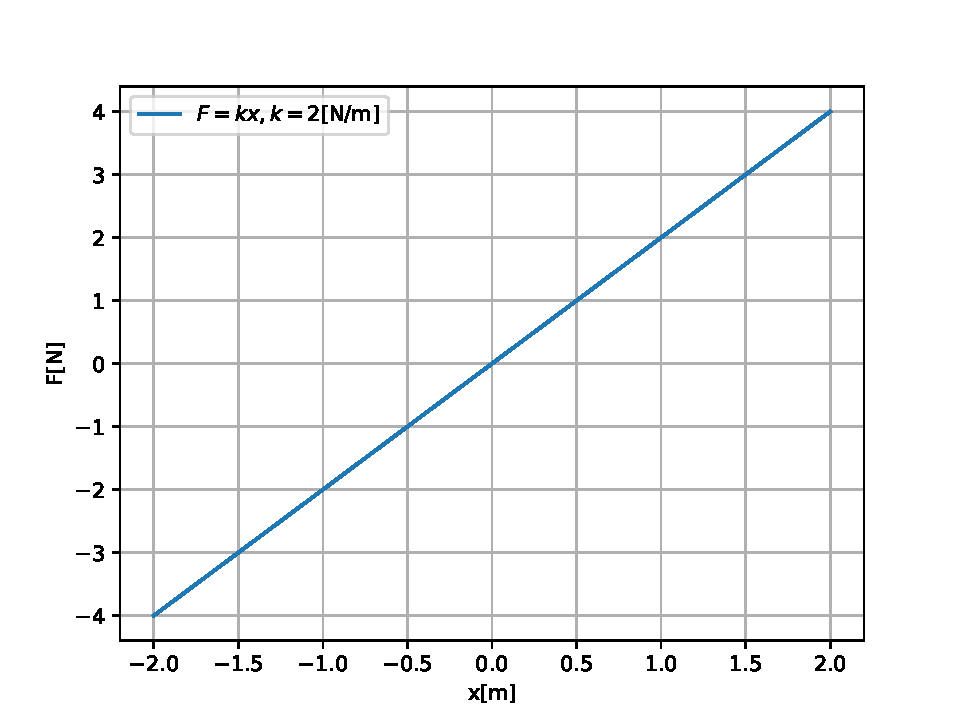
\includegraphics[width = 0.8\columnwidth]{fook_graph.pdf}
		\caption{フックの法則のグラフによる表現}
		\label{fig:fook}
	\end{figure}

	% \subsubsection*{いろいろな例}


	
	% \subsection{具体的な数字の代わりの文字(定数)}
	% 再びフックの法則を考えましょう。
	% \begin{itembox}[l]{(例)フックの法則(再掲)}
	% 	ばねが$x$だけ伸びたときのばねの引っ張る力(張力)Fは次のような式で与えられる。
	% 	\begin{equation*}
	% 	F = kx
	% 	\end{equation*}
	% 	ただし、ばねの材質などによって決まる$k$はばね定数である。
	% \end{itembox}
	% ここで、前節で触れなかった文字、$k$について考えてみましょう。
	
	
	
	
\end{document}

